\subsubsection{Company}
Meanwhile companies can also access the site to gain access to students. For example a recruiter from Netcraft, Sally, wishes to sign up in order to find students for placements.
  \paragraph{Sign up:}
    If Netcraft had not yet registered as a company, then the Sally must sign up on Netcrafts behalf, which is very similar to the student signup page.
    Since Netcraft already exists then Sally must request that another admininistrator adds her by signing in and clicking on the new administrator button.

  \paragraph{Contacts:}
    Sally decides that she wishes to be contacted by students regarding job oppourtunities so adds her details to the company contacts in the top left hand corner. This very nicely comes up with an inplace form for Sally to fill out. However since Netcraft already has many company contacts she does not automatically appear at the top of the list. 
    %TODO Sally is alerted by tooltip taht she can reorder company contacts.
    She then clicks on all contacts and drags herself up to the top of the list in order to be displayed, when returning to the page she now notices that she's top of the list.
    Students viewing this page can then email any of the contacts since they must disclose their email addresses.

  \paragraph{Events and Placements:}
    Sally decides that it might be a good idea to post that Netcraft is offering six month industrial placements and so clicks on the new placement button. 
    She receives important notices from the departments she's registered to that she reads and makes note of and then procedes to create the placement which once submitted will be approved via a department admin before shown on their site.
    Similarly Sally can do the exact same thing with events.
  
  \paragraph{Students:}
    After creating placements and events Sally decides she wants to browse students to find exceptional candidates she can contact herself. She clicks on students on the navigation bar and is greeted by a list of students. Note that any students who have decided to black Netcraft will never appear in this list, nor will deactivated students.
    %TODO MAKE SURE FILTERING IS IMPLEMENTED, and JACK has Perl as a skill
    Since she knows Netcraft will be recruiting for Perl developers, she specifically types Perl into the skills filter
    and filters the list down to the students who have it as a skill.
    %TODO print screen
    She can then browse their profiles, which is a reduced version of the student view. Liking what she see's Sally can then choose to download Jack's CV to her computer or view it online with the preview icon. 

    %TODO CLICK ON MAIL ICON
    Liking what she sees Sally then chooses to invite Jack to interview, by clicking on the contact student button. She then sends an email from her account to his address which he can reply to if he wants. 

    \begin{figure}[H]\centering
    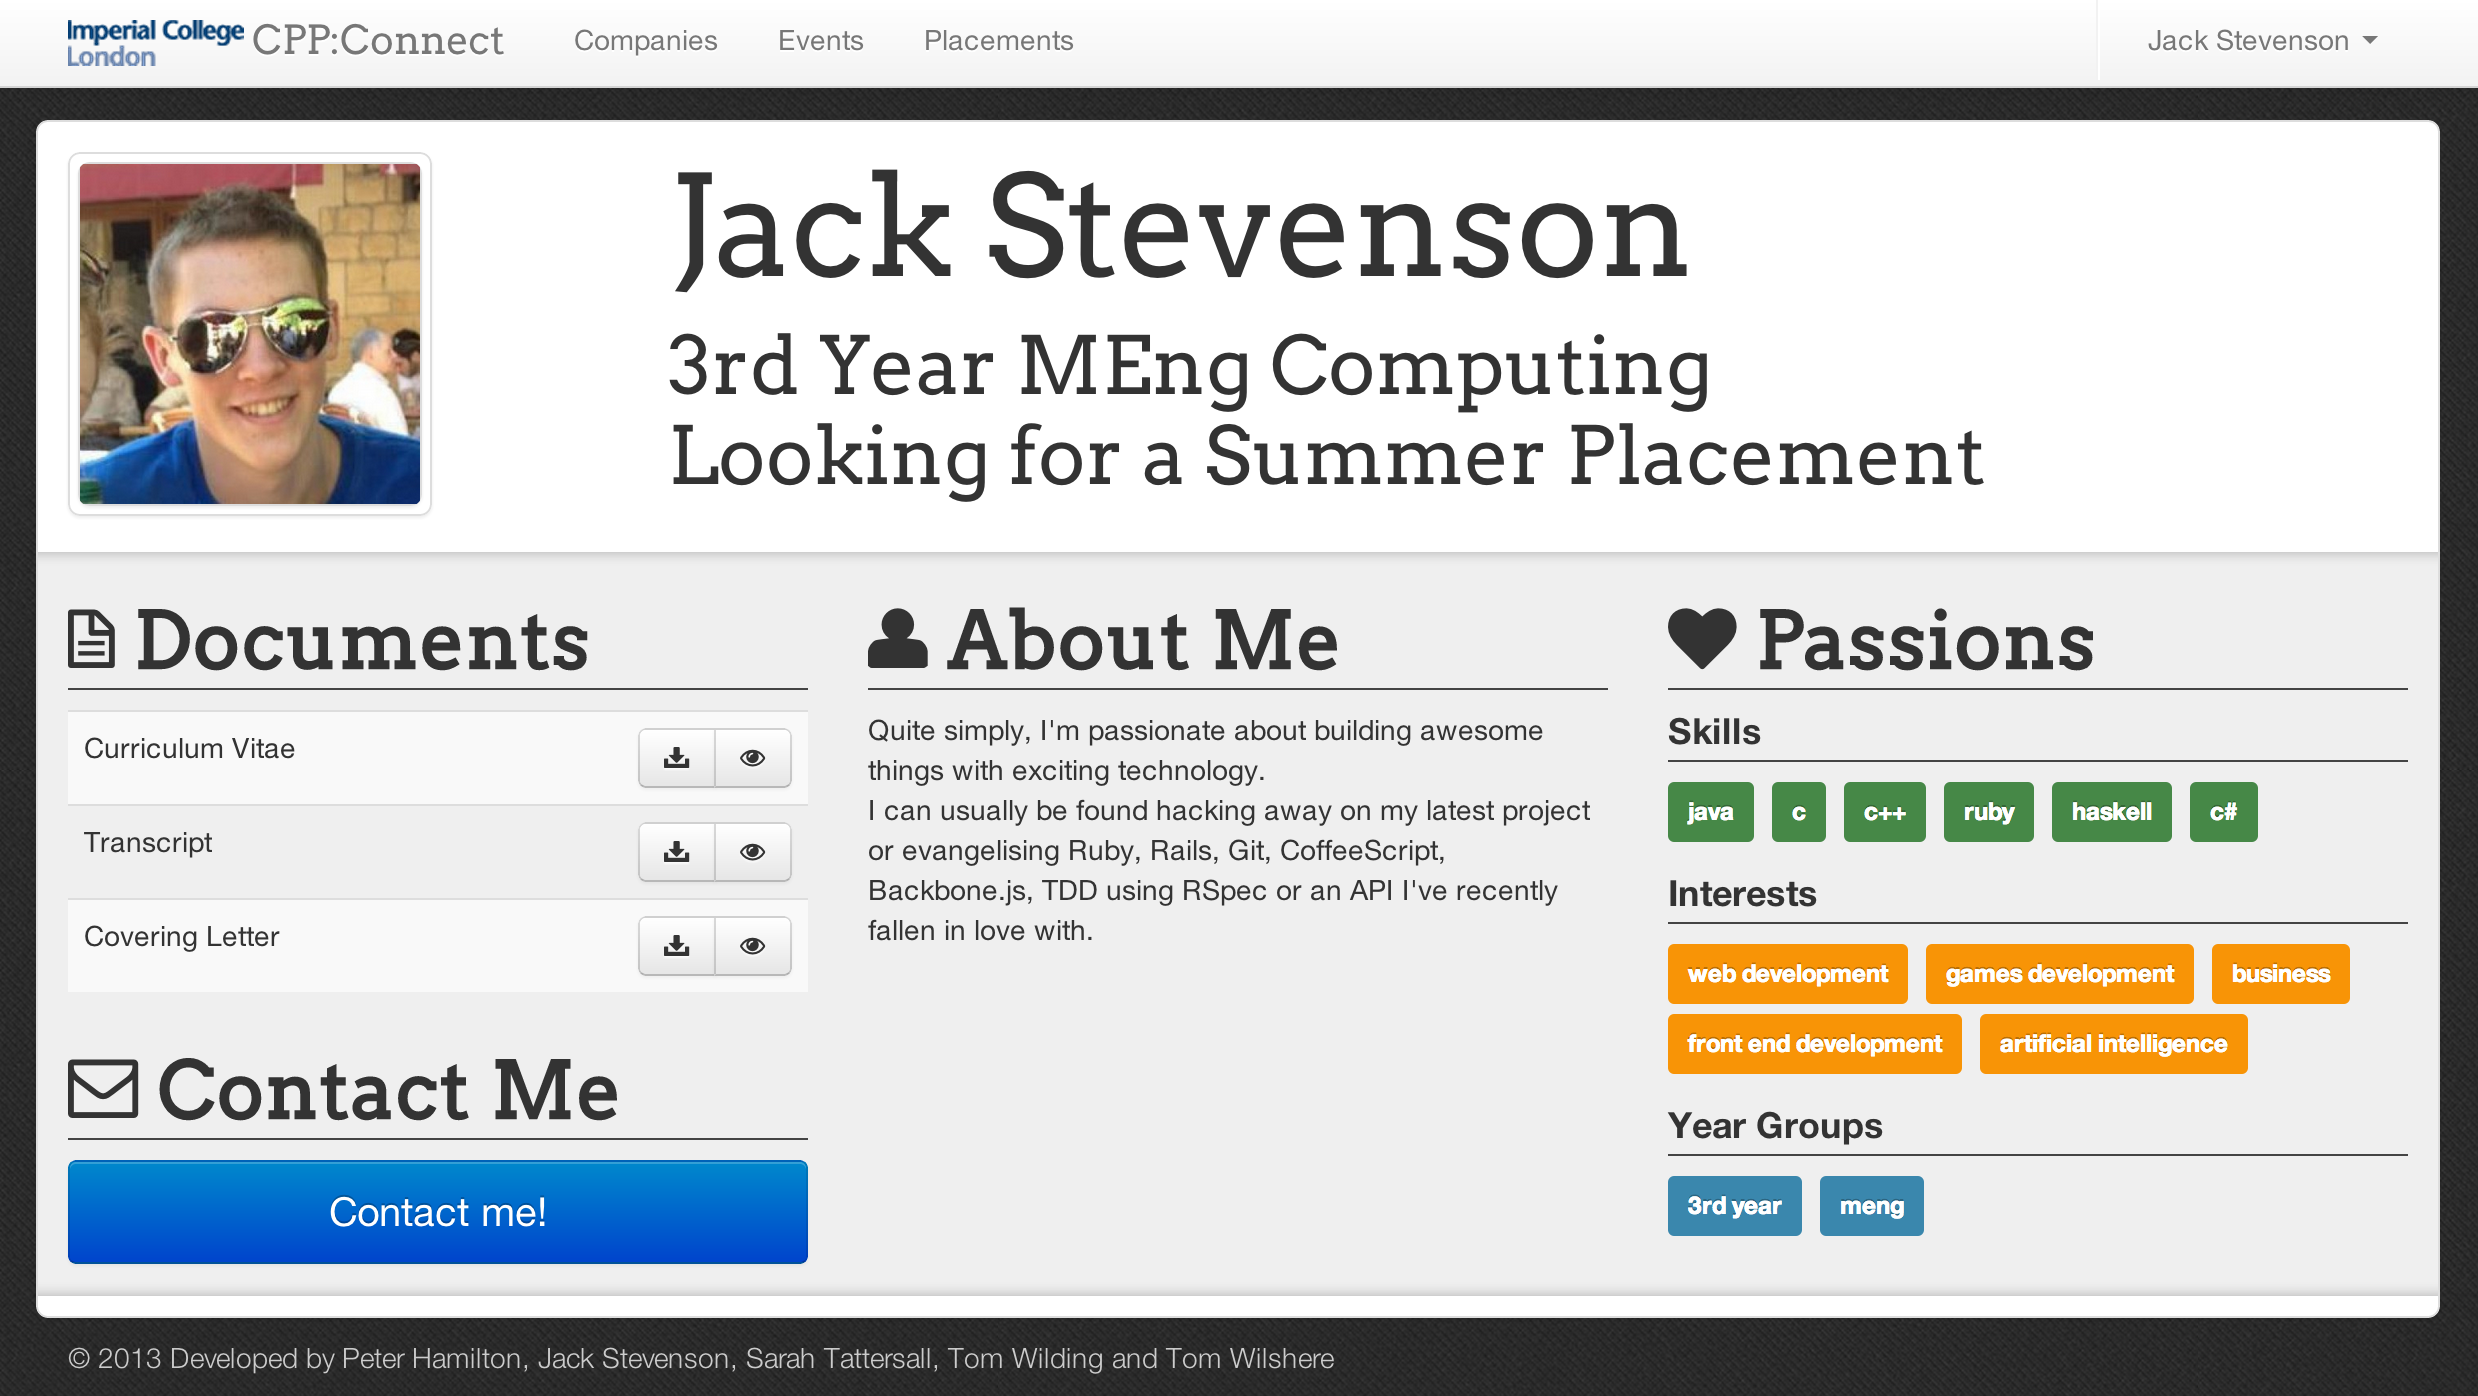
\includegraphics[scale=0.3]{images/user_experiences/company/jack_profile}
    \end{figure}

  \paragraph{Emails:}
    Being a member of the Corporate Partnership Program also entitles Netcraft to be able to contact a departments students via email. Sally can create emails to inform students of exciting scholarships Netcraft are offering, or news about the company.

    ****************** TODO ******************
    Write about an email!

    %TODO A little more
